\title{Лекция 22\\Принципы многоагентной обработки баз знаний}
\author[]{Шункевич Д.В.}
\institute[]{Белорусский государственный университет информатики и радиоэлектроники}

\begin{frame}
	\titlepage
\end{frame}

\begin{frame}{\\Содержание лекции}
	\topline
	\justifying
	Понятие sc-агента, классификация sc-агентов. Принципы реализации многоагентной обработки знаний в семантической памяти. Спецификация действий sc-агентами, пример решения задачи коллективом агентов. Пользователь компьютерной системы как sc-агент. Спецификация sc-агентов, пример описания в базе знаний. Атомарные и неатомарные sc-агенты, иерархия sc-агентов.
\end{frame}

\begin{frame}{\\Понятие sc-агента}
		\topline
	\justifying
	\begin{SCn}
		\scnheader{sc-агент}
		\begin{scnindent}
			\scnidtf{единственный вид субъектов, выполняющих преобразования в sc-памяти}
			\scnidtf{субъект, способный выполнять действия в sc-памяти, принадлежащие некоторому определенному классу логически атомарных действий}
		\end{scnindent} \vspace{5mm}
	Логическая атомарность выполняемых sc-агентом действий предполагает, что каждый sc-агент реагирует на соответствующий ему класс ситуаций и/или событий, происходящих в sc-памяти, и осуществляет определенное преобразование sc-текста, находящегося в семантической окрестности обрабатываемой ситуации и/или события.
	\end{SCn}
\end{frame}
\begin{frame}{\\Понятие абстрактного sc-агента}
		\topline
	\justifying
	
	Предполагая, что копии одного и того же sc-агента или функционально эквивалентные sc-агенты могут работать в разных ostis-системах, будучи при этом физически разными sc-агентами, то целесообразно рассматривать свойства и классификацию не sc-агентов, а классов функционально эквивалентных sc-агентов, которые будем называть абстрактными sc-агентами. Под абстрактным sc-агентом понимается некоторый класс функционально эквивалентных sc-агентов, разные экземпляры (т.е. представители) которого могут быть реализованы по-разному.
	
\end{frame}
\begin{frame}{\\Классификация абстрактных sc-агентов}
		\topline
	\justifying
	\begin{SCn}
		\scnheader{абстрактный sc-агент}
		\begin{scnrelfromset}{разбиение}
			\scnitem{неатомарный абстрактный sc-агент}
			\scnitem{атомарный абстрактный sc-агент}
		\end{scnrelfromset}
		\begin{scnrelfromset}{разбиение}
			\scnitem{внутренний абстрактный sc-агент}
			\scnitem{эффекторный абстрактный sc-агент}
			\scnitem{рецепторный абстрактный sc-агент}
		\end{scnrelfromset}
		\begin{scnrelfromset}{разбиение}
			\scnitem{абстрактный sc-агент, не реализуемый на Языке SCP}
			\scnitem{абстрактный sc-агент, реализуемый на Языке SCP}
		\end{scnrelfromset}
	\end{SCn}
\end{frame}
\begin{frame}{}
		\topline
	\justifying
	\begin{SCn}
		\begin{scnrelfromset}{разбиение}
			\scnitem{абстрактный sc-агент интерпретации scp-программ}
			\scnitem{абстрактный программный sc-агент}
			\scnitem{абстрактный sc-метаагент}
		\end{scnrelfromset}
		\begin{scnrelfromset}{разбиение}
			\scnitem{платформенно-зависимый абстрактный sc-агент \\
			 \scnsuperset{абстрактный sc-агент, не реализуемый на Языке SCP}
		}
				
			\scnitem{платформенно-независимый абстрактный sc-агент}
		\end{scnrelfromset}
	\end{SCn}
\end{frame}

\begin{frame}{\\Абстрактный неатомарный sc-агент}
		\topline
	\justifying
	\scnheader{неатомарный абстрактный sc-агент}
	\scnrelfrom{пояснение}{Под неатомарным абстрактным sc-агентом понимается абстрактный sc-агент, который декомпозируется на коллектив более простых абстрактных sc-агентов, каждый из которых в свою очередь может быть как атомарным абстрактным sc-агентом, так и неатомарным абстрактным sc-агентом. При этом в каком либо варианте декомпозиции абстрактного sc-агента* дочерний неатомарный абстрактный sc-агент может стать атомарным абстрактным sc-агентом, и реализовываться соответствующим образом.}
\end{frame}

\begin{frame}{\\Абстрактный атомарный sc-агент}
		\topline
	\justifying
	\scnheader{атомарный абстрактный sc-агент}
	\scnrelfrom{пояснение}{Под атомарнымабстрактным sc-агентомпонимается абстрактный sc-агент, для которого уточняется платформа его реализации, т.е. существует соответствующая связка отношения программа sc-агента*.}
	\begin{scnrelfromset}{разбиение}
		\scnitem{платформенно-независимый абстрактный sc-агент}
		\scnitem{платформенно-зависимый абстрактный sc-агент}
	\end{scnrelfromset}
\end{frame}

\begin{frame}{\\Внутренний абстрактный sc-агент}
		\topline
	\justifying
	\scnheader{внутренний абстрактный sc-агент}
	\scnrelfrom{пояснение}{Каждый внутренний абстрактный sc-агент обозначает класс sc-агентов, которые реагируют на события в sc-памяти и осуществляют преобразования исключительно в рамках этой же sc-памяти.}
\end{frame}

\begin{frame}{\\Эффекторный абстрактный sc-агент}
		\topline
	\justifying
	\scnheader{эффекторный абстрактный sc-агент}
	\scnrelfrom{пояснение}{Каждый эффекторный абстрактный sc-агент обозначает класс sc-агентов, которые реагируют на события в sc-памяти и осуществляют преобразования во внешней относительно данной ostis-системы среде.}
\end{frame}

\begin{frame}{\\Рецепторный абстрактный sc-агент}
		\topline
	\justifying
	\scnheader{рецепторный абстрактный sc-агент}
	\scnrelfrom{пояснение}{Каждый рецепторный абстрактный sc-агент обозначает класс sc-агентов, которые реагируют на события во внешней относительно данной ostis-системы среде и осуществляют преобразования в памяти
		данной системы.}
\end{frame}

\begin{frame}{Абстрактный sc-агент, не реализуемый на\\ Языке SCP}
		\topline
	\justifying
	\scnheader{абстрактный sc-агент, не реализуемый на Языке SCP}
	\scnrelfrom{пояснение}{Каждый абстрактный sc-агент, не реализуемый на Языке SCP должен быть реализован на уровне платформы интерпретации sc-моделей, в том числе, аппаратной. К таким абстрактным sc-агентам относятся абстрактные sc-агенты интерпретации scp-программ, а также эффекторные и рецепторные абстрактные sc-агенты.}
	
\end{frame}

\begin{frame}{Абстрактный sc-агент, реализуемый на\\ Языке SCP}
		\topline
	\justifying
\scnheader{абстрактный sc-агент, реализуемый на Языке SCP}
\scnrelfrom{пояснение}{Каждый абстрактный sc-агент, реализуемый на Языке SCP может быть реализован на Языке SCP, то есть платформенно-независимом уровне, но при необходимости, может реализовываться и на уровне платформы, например, с целью повышения производительности.}
\end{frame}

\begin{frame}{Абстрактный sc-агент интерпретации scp-программ}
		\topline
	\justifying
	\scnheader{абстрактный sc-агент интерпретации scp-программ}
	\scnrelfrom{пояснение}{К абстрактным sc-агентам интерпретации scp-программ относятся не реализуемые на платформеннонезависимом уровне абстрактные sc-агенты, обеспечивающие интерпретацию scp-программ и scp-метапрограмм, в том числе создание scp-процессов, собственно интерпретацию scp-операторов, а также другие вспомогательные действия. По сути, агенты данного класса обеспечивают работу sc-агентов более высоких уровней (программных sc-агентов и sc-метаагентов), реализованных на Языке SCP, в частности, обеспечивают соблюдение указанными агентами общих принципов синхронизации.}
\end{frame}

\begin{frame}{\\Абстрактный программный sc-агент}
		\topline
	\justifying
	\scnheader{абстрактный программный sc-агент}
	\scnrelfrom{пояснение}{К абстрактным программным sc-агентам относятся все абстрактные sc-агенты, обеспечивающие основной функционал системы, то есть ее возможность решать те или иные задачи. Агенты данного класса должны работать в соответствии с общими принципами синхронизации деятельности субъектов в sc-памяти.}
\end{frame}

\begin{frame}{\\Абстрактный sc-метаагент}
		\topline
	\justifying
	\scnheader{абстрактный sc-метаагент}
	\scnrelfrom{пояснение}{Задачей абстрактных sc-метаагентов является координация деятельности абстрактных программных sc-агентов, в частности, решение проблемы взаимоблокировок. Агенты данного класса могут быть реализованы на Языке SCP, однако для синхронизации их деятельности используются другие принципы, соответственно, для реализации таких агентов требуется Язык SCP другого уровня, типология операторов которого полностью аналогична типологии scp-операторов, однако эти операторы имеют другую операционную семантику, учитывающую отличия в принципах синхронизации (работы с блокировками*). Программы такого языка будем называть scp-метапрограммами, соответствующие им процессы в sc-памяти – scp-метапроцессами, операторы – scp-метаоператорами.}
\end{frame}

\begin{frame}{Платформенно-зависимый абстрактный sc-агент}
		\topline
	\justifying
	\scnheader{платформенно-зависимый абстрактный sc-агент}
	\scnrelfrom{пояснение}{К платформенно-зависимым абстрактным sc-агентам относят атомарные абстрактные sc-агенты, реализованные ниже уровня sc-моделей, т.е. не на Языке SCP, а на каком-либо другом языке описания программ. Существуют sc-агенты, которые принципиально должны быть реализованы на платформенно-зависимом уровне, например, собственно sc-агенты интерпретации sc-моделей или рецепторные и эффекторные sc-агенты, обеспечивающие взаимодействие с внешней средой.}
\end{frame}

\begin{frame}{Платформенно-независимый абстрактный sc-агент}
		\topline
	\justifying
	\scnheader{платформенно-независимый абстрактный sc-агент}
	\scnrelfrom{пояснение}{К платформенно-независимым абстрактным sc-агентам относят атомарные абстрактные sc-агенты, реализованные на базовом языке программирования Технологии OSTIS, т.е. на Языке SCP. При описании платформенно-независимых абстрактных sc-агентов под платформенной независи мостью понимается платформенная независимость с точки зрения Технологии OSTIS , поскольку атомарные sc-агенты, реализованные на языке SCP могут свободно переноситься с одной платформы интерпретации sc-моделей на другую. При этом языки программирования, традиционно считающиеся платформенно-независимыми в данном случае не могут считаться таковыми.}
\end{frame}

\begin{frame}{Принципы реализации многоагентной обработки знаний в семантической памяти}
		\topline
	\justifying
	
	Одной из важных особенностей многоагентного подхода к решению задач является возможность параллельного решения различных задач, что в свою очередь, предполагает параллельность выполнения соответствующих информационных процессов.\\
	Понятия действие в sc-памяти, и процесс в sc-памяти являются синонимичными, поскольку все процессы, протекающие в sc-памяти, являются осознанными и выполняются каким-либо sc-агентами.\\
	Для синхронизации выполнения процессов в sc-памяти предлагается использовать механизм блокировок, построенный на основе существующих алгоритмов синхронизации информационных процессов в традиционных системах.
\end{frame}

\begin{frame}{\\Отношение блокировка}
	\topline
\justifying
\begin{SCn}
	\scnheader{отношение блокировка*}
	\scniselement{бинарное отношение}
	\scnheader{тип блокировки}
	\scnhaselement{полная блокировка}
	\scnhaselement{блокировка на любое изменение}
	\scnhaselement{блокировка на удаление}
\end{SCn}
Отношение блокировка* связывает знаки действий в sc-памяти со знаками структур, которые содержат элементы, заблокированные на время выполнения данного действия. Первым компонентом связок отношения блокировка* является знак действия в sc-памяти, вторым – знак заблокированной структуры.
\end{frame}
\begin{frame}{\\}
		\topline
	\justifying
	\vspace{3em}
	\begin{figure}[H]
		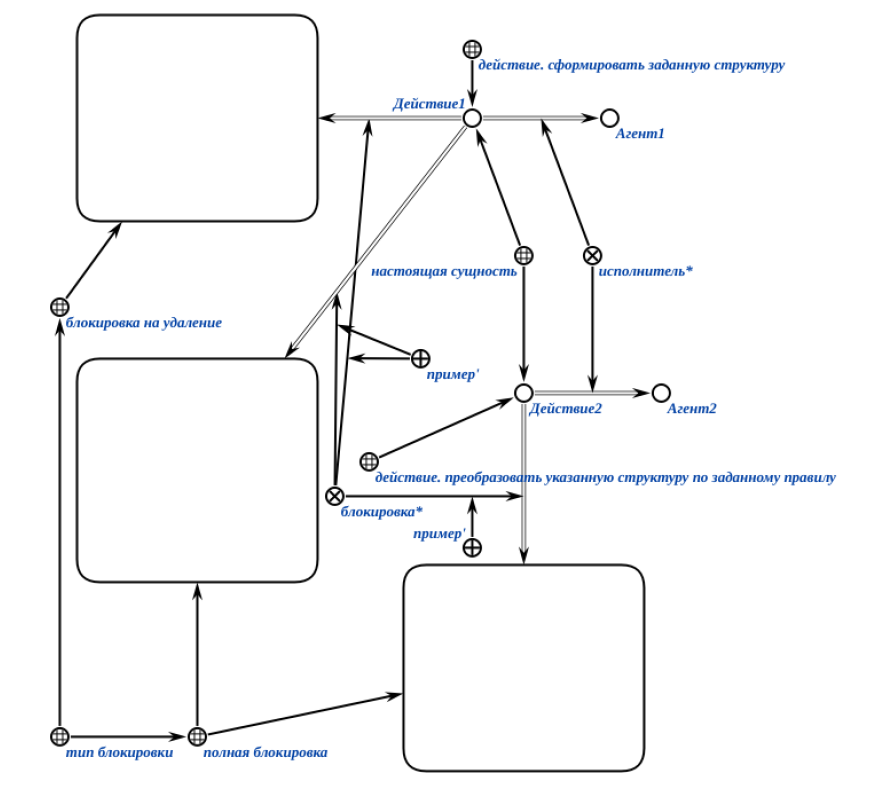
\includegraphics[scale=0.25]{./figures/sd_multiagent_processing/blocking_example.png}
		\caption{Пример использования блокировок}
	\end{figure}
\end{frame}

\begin{frame}{\\Полная блокировка}
		\topline
	\justifying
	\begin{SCn}
		\scnheader{полная блокировка}
		\scnrelfrom{пояснение}{Каждая структура, принадлежащая множеству полная блокировка содержит sc-элементы, просмотр и изменение которых запрещены всем sc-агентам, кроме собственно sc-агента, выполняющего соответствующее данной структуре действие в sc-памяти, связанное с ней отношением блокировка*. Для того, чтобы исключить возможность реализации sc-агентов, которые могут внести изменения в конструкции, описывающие блокировки других sc-агентов, все элементы этих конструкций, в том числе, сам знак структуры, содержащей заблокированные sc-элементы и связки отношения блокировка*, связывающие эту структуру и конкретное действие в sc-памяти, добавляются в полную блокировку, соответствующую данному действию в sc-памяти.}

	\end{SCn}
\end{frame}

\begin{frame}{\\Блокировка на любое изменение}
		\topline
	\justifying
	\begin{SCn}
		\scnheader{блокировка на любое изменение}
		\scnrelfrom{пояснение}{Каждая структура, принадлежащая множеству блокировка на любое изменение содержит sc-элементы, изменение (физическое удаление, добавление инцидентных sc-коннекторов, физическое удаление самих sc-элементов, изменение содержимого в случае файла) которых запрещено всем sc-агентам, кроме собственно sc-агента, выполняющего соответствующее данной структуре действие в sc-памяти, связанное с ней отношением блокировка*. Однако не запрещен просмотр (чтение) этих sc-элементов любым sc-агентом.}
		
	\end{SCn}
\end{frame}

\begin{frame}{\\Блокировка на удаление}
		\topline
	\justifying
	\begin{SCn}
		\scnheader{блокировка на удаление}
		\scnrelfrom{пояснение}{Каждая структура, принадлежащая множеству блокировка на удаление содержит sc-элементы, удаление которых запрещено всем sc-агентам, кроме собственно sc-агента, выполняющего соответствующее данной структуре действие в sc-памяти, связанное с ней отношением блокировка*. Однако не запрещен просмотр (чтение) этих sc-элементов любым sc-агентом, добавление инцидентных sc-коннекторов.}
		
	\end{SCn}
\end{frame}


\begin{frame}{\\Спецификация действий sc-агентами}
		\topline
	\justifying
	\begin{SCn}
		\scnheader{действие в sc-памяти}
		\scnrelfrom{пояснение}{Каждое действие в sc-памяти обозначает некоторое преобразование, выполняемое некоторым sc-агентом (или коллективом sc-агентов) и ориентированное на преобразование sc-памяти.}
		\scnsuperset{действие в sc-памяти, инициируемое вопросом}
		\scnsuperset{действие редактирования базы знаний ostis-системы}
		\scnsuperset{действие установки режима ostis-системы}
		\scnsuperset{действие редактирования файла, хранимого в sc-памяти}
		\scnsuperset{действие интерпретации программы, хранимой в sc-памяти }
	\end{SCn}
\end{frame}

\begin{frame}{Пользователь компьютерной системы как sc-агент}
		\topline
	\justifying
	Пользователь ostis-системы не может сам непосредственно выполнить какое-либо действие в sc-памяти, но он может средствами пользовательского интерфейса инициировать построение (генерацию, формирование в sc-памяти) sc-текста, являющегося спецификацией действия в sc-памяти, выполняемого либо одним атомарным sc-агентом за один акт, либо одним атомарным sc-агентом за несколько актов, либо коллективом sc-агентов (неатомарным sc-агентом). В спецификации каждого такого действия в sc-памяти, инициированного пользователем, этот пользователь указывается как заказчик этого действия. Таким образом, пользователь ostis-системы может рассамтриватся как некий sc-агент выполняющий действия в sc-памяти при помощи других sc-агентов.
\end{frame}

